%----------------------------------------------------------------------------------------
%	PACKAGES AND DOCUMENT CONFIGURATIONS
%----------------------------------------------------------------------------------------
\documentclass[journal]{IEEEtran}
\usepackage{amsmath} % Required for some math elements
\usepackage{hyperref}
\usepackage[table,xcdraw]{xcolor}
\usepackage{lipsum} 
\usepackage{cite}
\usepackage{graphicx} % Required for the inclusion of images
\usepackage{algorithmic}
\usepackage{array}
\usepackage{bookmark}

\interdisplaylinepenalty=2500 %Note that the amsmath package sets \interdisplaylinepenalty to 10000 thus preventing page breaks from occurring within multiline equations. Use: \interdisplaylinepenalty=2500 after loading amsmath to restore such page breaks as IEEEtran.cls normally does

\hypersetup{ %color attributes of citation, link, etc.
    colorlinks=orange,
    linkcolor=cyan,
    filecolor=gray,      
    urlcolor=cyan,
    citecolor=cyan,
}
%----------------------------------------------------------------------------------------
%	DOCUMENT INFORMATION
%----------------------------------------------------------------------------------------
\title{RESE412 - Project 1 Report \\ Sizing of a Renewable Microgrid}
\author{Daniel Eisen}
\date{\today}

\begin{document}
\onecolumn
\maketitle
\tableofcontents
%----------------------------------------------------------------------------------------
%	DOCUMENT CONTENT
%----------------------------------------------------------------------------------------
\twocolumn
\section{Introduction}
  \IEEEPARstart{T}{his} project and report describes the process and presents the results of sizing a renewable energy generation solution for a relatively isolated small residential settlement. After the location and environmental circumstance was characterised, an incremental analysis was undertaken with the use of Simulink simulation modelling. Each household model was first individually sized for using a nanogrid approach for both solar and wind and had their performance documented. Then for microgrid integration, two scenarios were modelled; first the distributed model of interconnected individual nanogrids then a centralised generation topology.
  
  The goal in doing this approach is to build a greater understanding of the energy requirement of such a settlement, evaluate the comparative cost and efficacy of the various approach's in designing a long term standalone, renewable energy solution for such a community and the drawbacks/caveats and issue associated and encountered throughout. 

\section{Environmental Analysis}
In order to design the necessary to serve the settlement, influence that the environment will have must be taken into account and characterised/considered. Firstly the immediate topology and how it will affect total hours of available sun, wind obstruction via trees, and space requirements for distancing turbines, or placing solar panels.

The site chosen for this settlement is a ridge in the south-west of the Wellington region, specifically at $-41.335^{\circ}, 174.705^{\circ}$, with a planned 6 plots for residential households though this report will only look at modelling an initial settlement of size 4.
        \subsection{Topological Discussion}
        \begin{figure}[h!]
                \centering
                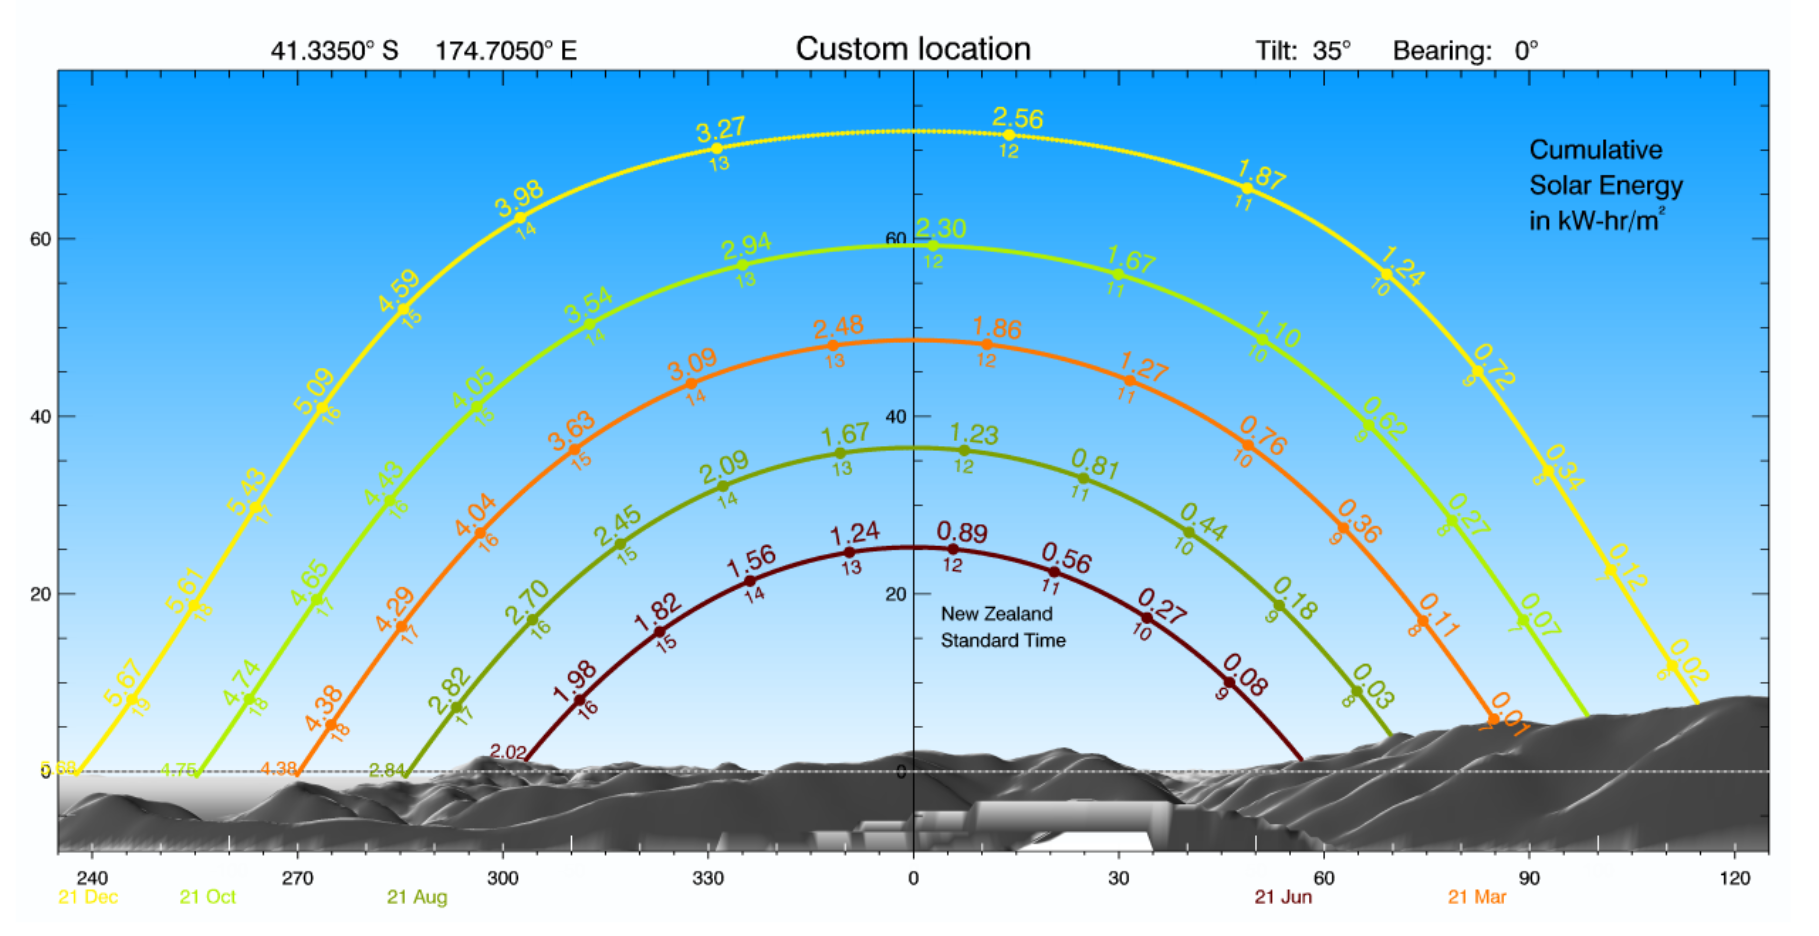
\includegraphics[width=0.75\linewidth]{fig/niwa_solarview.png}
                \caption{NIWA SolarView of Location}
                \label{solarview}
        \end{figure}

        The site is a flat, treeless ridge so environmental obstructions, see appendix \ref{ap:location}, to wind or solar are completely minimal and the only considerations that would need to be taken into account are placement during construction; concerning panel array placement (if not rooftop) and staggering turbine as to have them out of line with each other.

        Figure \ref{solarview} shows the the solar obstruction mapping from the north bearing. I can be seen that the rise time in summer is cut off to just before 6am, but more importantly in winter when solar irradiance is at a premium there is practically no restriction is the time between rise/set that there should theoretically be available sun. 

        These two observations; the lack of trees and minimal solar occluding hills/surrounding elevations indicates that investigations into the viability of both solar and wind as avenues of usable generation is feasible.
        
        \subsection{Solar Resources}
        NIWA provides the online tool SolarView\cite{solarview}. This was used to obtain detailed weather/environmental data about a specific location, taken from averaging past 25 years of collected data into a 'nominal' years worth of representative information. This requires the input of the locals coordinates and the indented panel tilt in degrees. By default SolarView will use the latitude but using an more optimal equation (from lat 25-50) \ref{tilt} a percentage of optimum capture of 71.1 can be achieved. For this location this is $\approx 35^{\circ}$.
        \begin{equation}
                Array_{tilt} = |lat|*0.76 + 3.1
                \label{tilt}
        \end{equation}

        From SolarView's provided data, the tilted irradiance is representative of what solar energy will be available to the installation for capture. From the years worth of data, a week was chosen to be the basis on which to characterise and size the nano/microgrids. This week is required to be 'averagely bad', meaning should not be an outlier in terms of terrible solar irradiance, having low average $W/m^2$ and a mix of slightly better and worse days. By sizing the installation for performing well in winter it can be taken for granted to work above specification across all the better months of the year.

        \begin{figure}[h!]
                \centering
                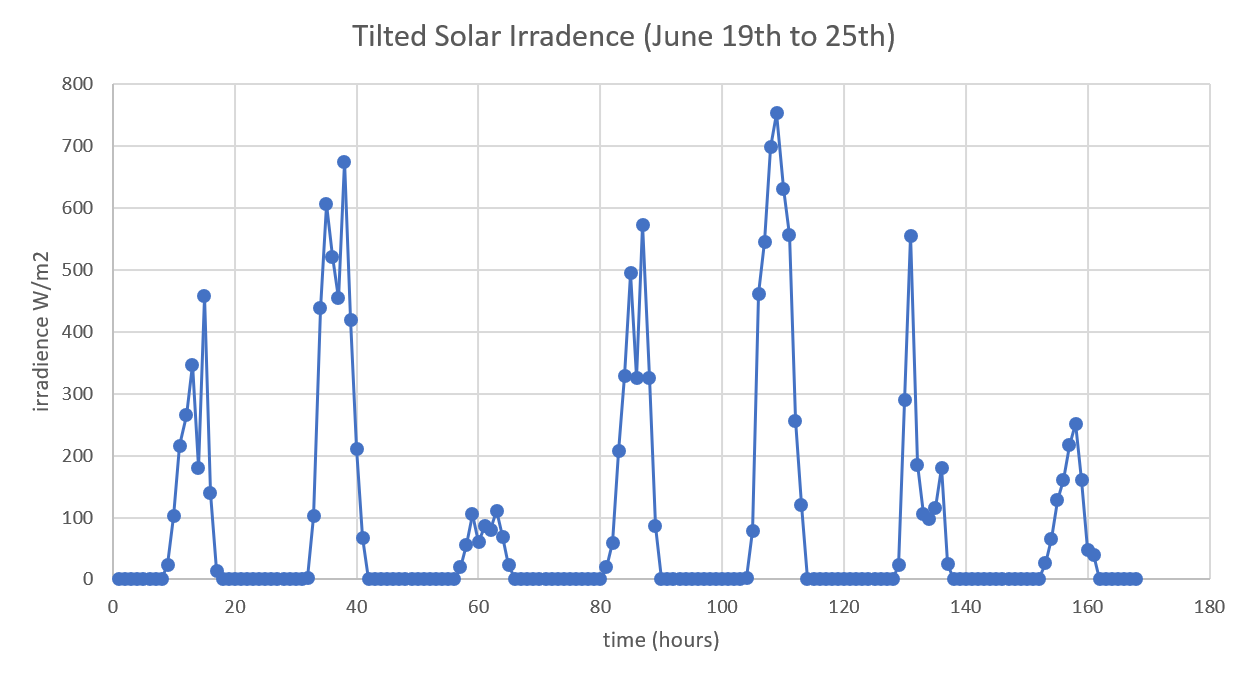
\includegraphics[width=0.75\linewidth]{fig/solar_irad.png}
                \caption{Solar Irradiance for chosen week}
                \label{solarweek}
        \end{figure}

        Taken the winter solstice (21 June) as a starting point, the 4 weeks of available solar irradiance surrounding were look over and 7 consecutive days were selected to meet the above defined specification. Resulting in the 7 days from the 19st to the 25th of June to represent an average week providing higher and lower days of available irradiance. Figure \ref{solarweek} shows this week, observing the low max irradiance of approximately $700W/$ and the spread of very low, medium and relatively higher days throughout the 7 days. This should provide a good basis for sizing a resilient installation.


        To quantify the solar resource into a singular usable number, this weeks data was transformed peak solar hours. Ie how many equivalent hours per day can the solar panel expect to receive the peak $1000 W/m^2$ of solar irradiance. This can either be done for each days average then taking the median, or by averaging the week then taking the peak solar hours. The latter was done in this case, doing either way yields very similar results, to result in \textbf{2.14 hrs}.

        \subsection{Wind Resources}
        To contrast and compare to the solar resource, the wind resource of the area is also taken into account. For ease of comparison the same week was chosen to use wind speed data from. 
        \begin{figure}[h!]
                \centering
                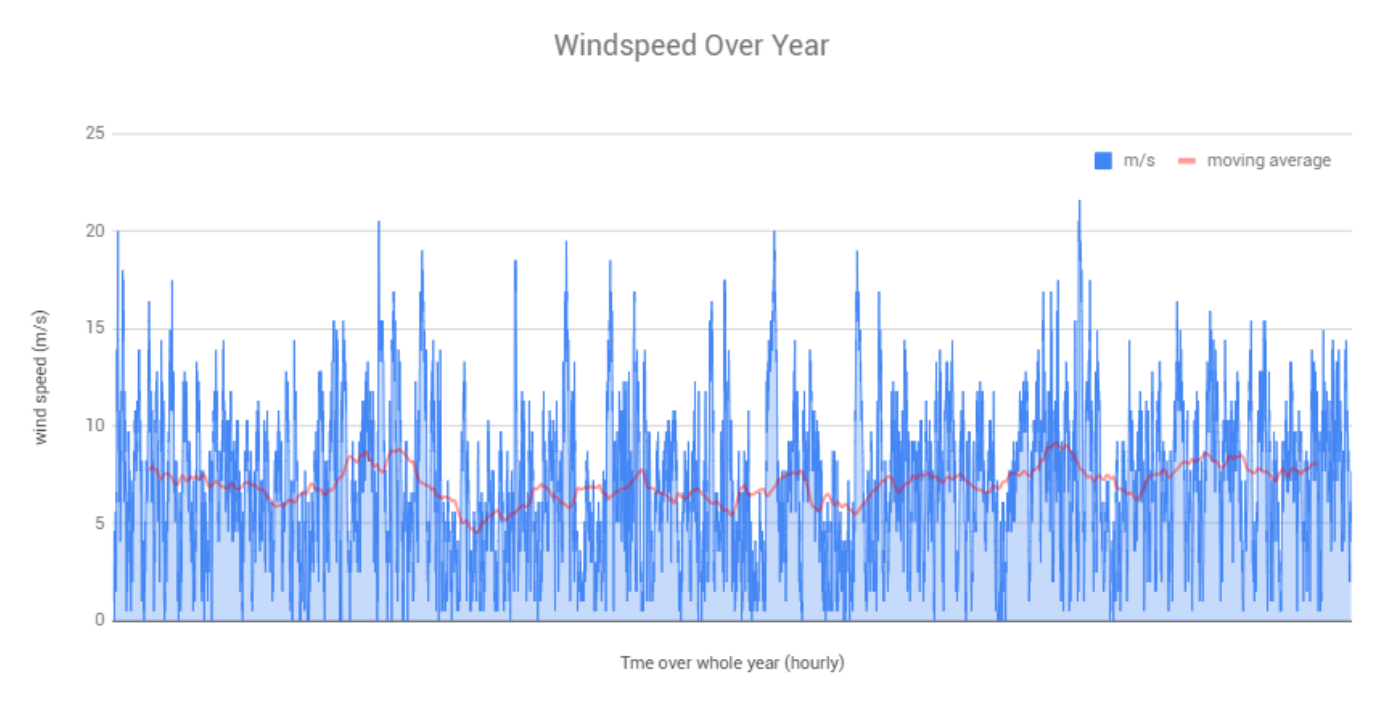
\includegraphics[width=0.75\linewidth]{fig/yearws.png}
                \caption{Year worth of windspeed}
                \label{yearwind}
        \end{figure}
        While this may not at first seem to be selected with the same rigour as the solar irradiance by observing the years data, see Figure \ref{yearwind}, it can be seen that for this location the windspeed level does not have any large scale cycling, possibly even a slight dip in the winter months maybe due to lower driving solar energy, so it can be treated as a fair and representative week for the year.
        
        \begin{figure}[h!]
                \centering
                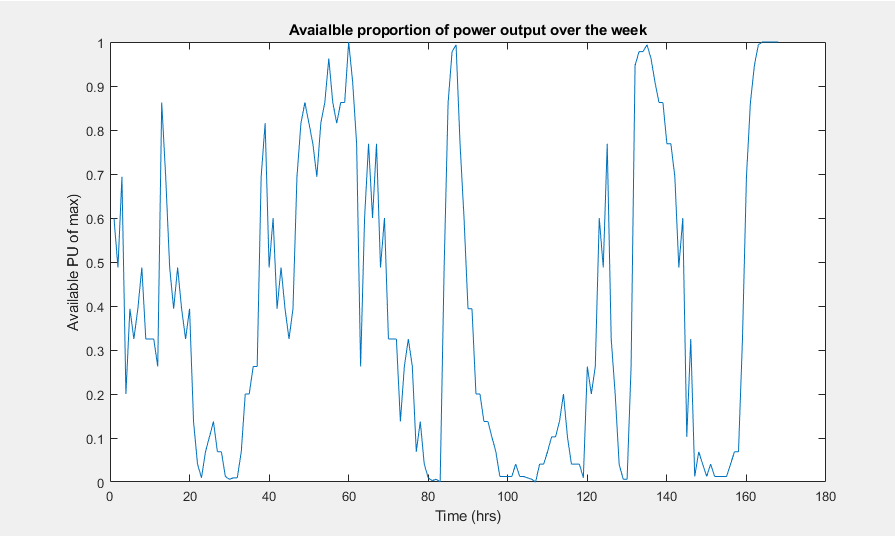
\includegraphics[width=0.7\linewidth]{fig/windPU.png}
                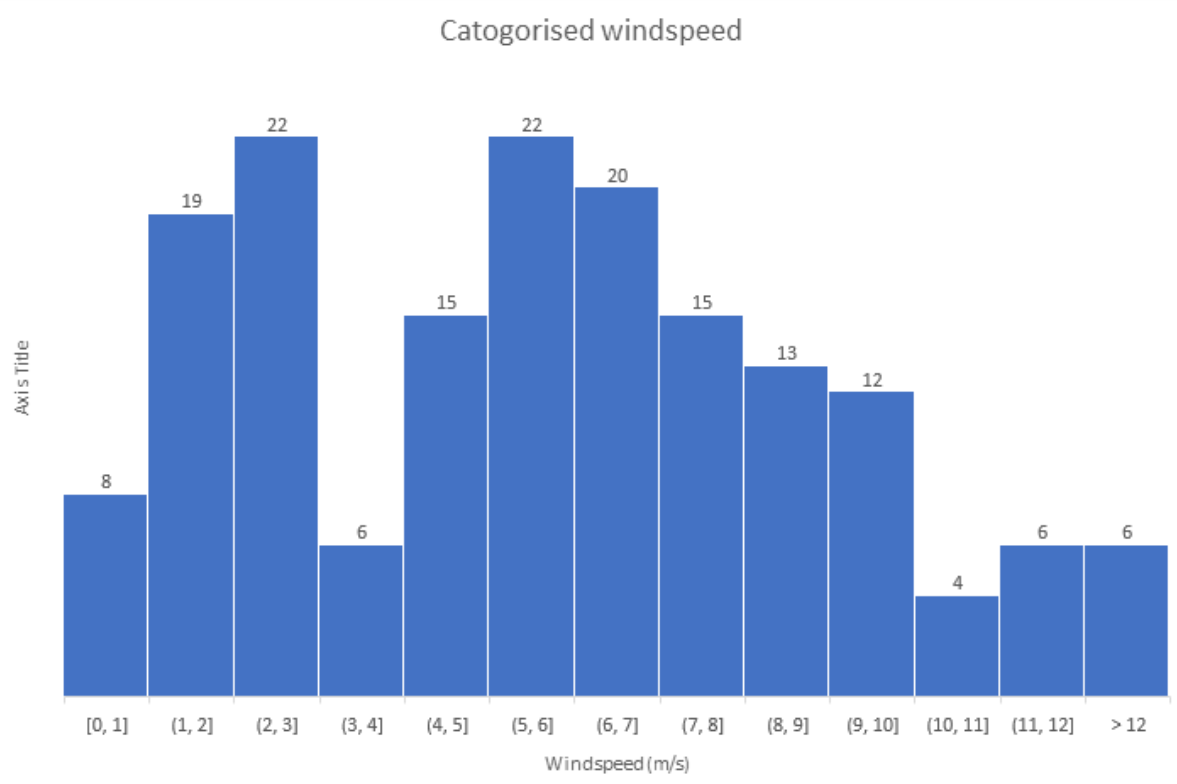
\includegraphics[width=0.7\linewidth]{fig/catorgws.png}
                \caption{Available turbine PU and windspeed histogram}
                \label{wind}
        \end{figure}
        In evaluating the wind resource the non linear and the turbine response has a maximum cap on its output at windspeeds greater than $12m/s$. See appendix \ref{ap:wind}. Figure \ref{wind} shows (right) the gross windspeed data binned into a histogram squashing speeds over-saturation and left is the result of running an interpolation of the data to the turbine response curve to retrieve its proportion of maximum power output over the week $(0.0 \rightarrow 1.1)$. Similarly to the peak sun hours previously discussed, this was used to determine the single value evaluation of the available wind resources. Summing the resulting vector and dividing by the number of days analysed results in a value of \textbf{9.43} equivalent hours of maximum turbine output. 
        
\section{Household Load Analysis}
Each home was characterised by simulating a week’s worth of usage, and averaging the integrated power usage to obtain a average daily usage, ie their energy consumption, scaled to kWhs. This way it accounts for slight variation across the days of the week.

\begin{table}[h!]
        \begin{center}
        \begin{tabular}{ll}
                \textbf{House} & \textbf{daily usage (kWh)}   \\
                \rowcolor[HTML]{C6EFCE} 
                2 & 17.88 \\
                \rowcolor[HTML]{FFEB9C} 
                3 & 19.78 \\
                \rowcolor[HTML]{FFC7CE} 
                4 & 16    \\
                \rowcolor[HTML]{BDD7EE} 
                5  & 39.59                       
        \end{tabular}
        \end{center}
\caption{Daily load requirements per household}
\label{tab:load}
\end{table}

\begin{figure}[h!]
        \centering
        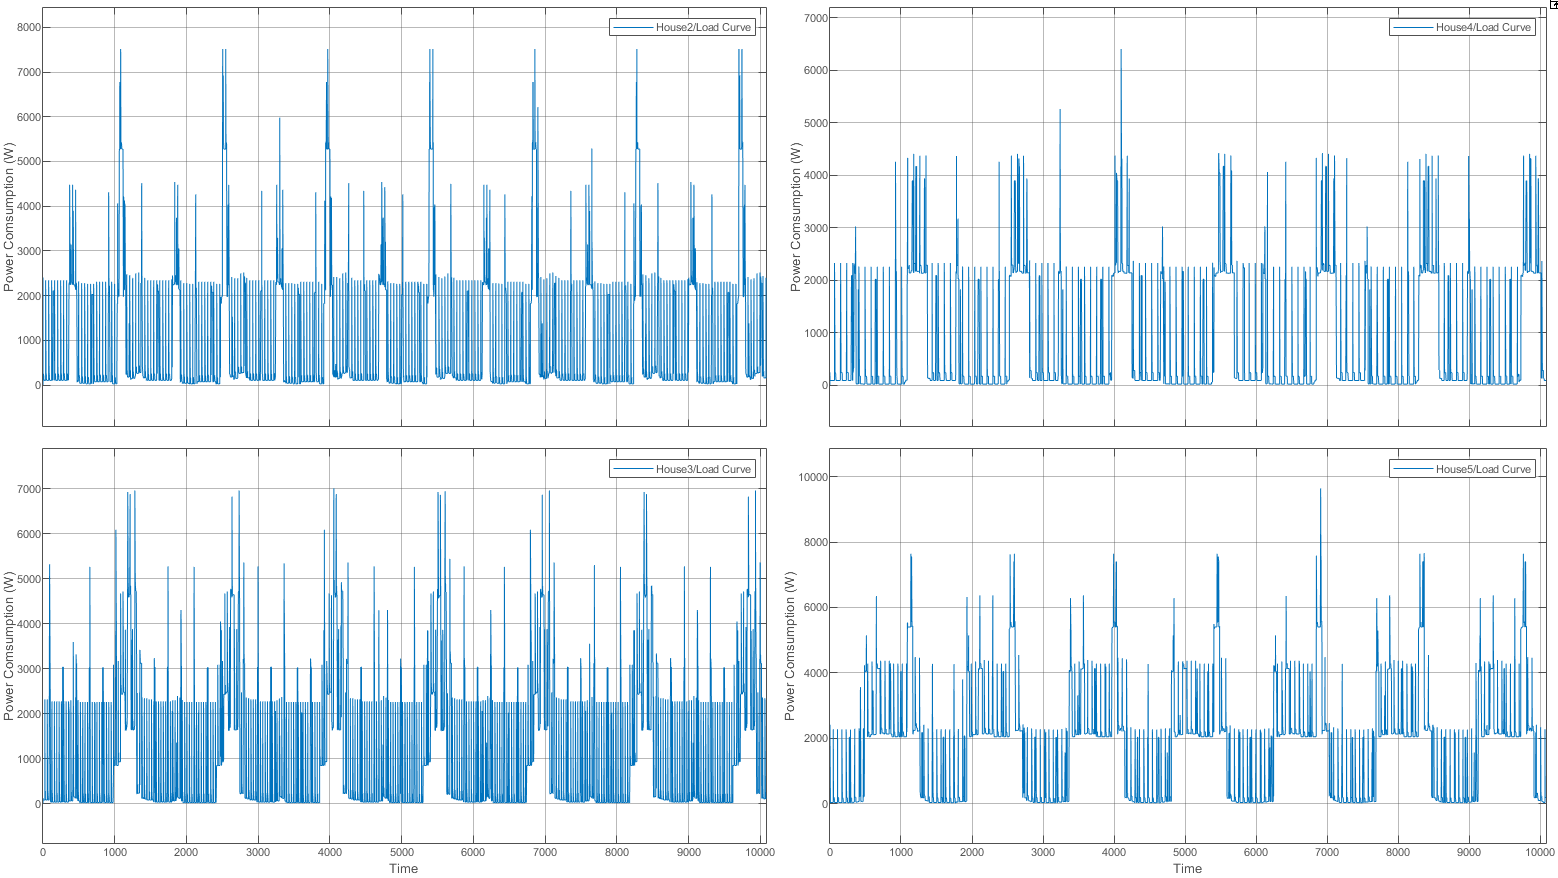
\includegraphics[width=0.75\linewidth]{fig/houseloads.png}
\caption{Household load}
\label{fig:load}
\end{figure}

The results of these simulation are shown above: Table \ref{tab:load} outlines the daily energy use per household as averaged over the week of simulation, indicating the necessity of individually sized solutions for each such that the nanogrids maximise they're efficiency, i.e. to avoid under/over-production.
These total usage values allow for the initial sizing of the generation, but without a look at the variation across daily usage in order to build an idea of how to smooth misalignment of generation to consumption with the right combination of generator and storage capacity. 
Some initial observations that will factor into the sizing are for example; house 5s much higher base load but also its consistency so high overlap with the solar generation period. Also house 4 with its majority consumption after the peak available sun, which will affect the needed storage in comparison to similar, but distributed loads.
\section{Nano-grid Sizing}
        \subsection{Initial Estimates}
                \subsubsection*{Storage}
                BMS storage set to meet 1 days worth of autonomy, required converting kWh to Ah at 240V.

                \subsubsection*{Photovoltaics}
                Step one, make initial estimate for sizing system with characterised available resources. Taking the daily usage and dividing the peak hours to get an initial panel wattage size for each home. 
                
                

                \subsubsection*{Wind Turbine}
                As with the photovoltaic sizing, the requirement is divided by the available out from the turbine to reach
                
                

        
        \subsection{Simulation and Meeting Requirements}
        

        \subsection{Notes on Hybrid}

\section{Resource Comparison}

\section{Nano grid Results}

\section{Microgrid}
        \subsection{Distributed}
        \subsection{Centralised}
        \subsection{Comparison}

\section{Conclusions and Recommendations}

\section{Reflecting on the Process}

\section{Reflecting on the Project}



\newpage
\onecolumn
\appendices
    \section{Location}
        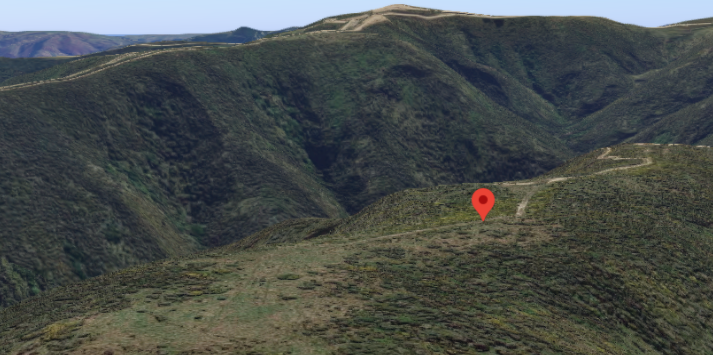
\includegraphics[width=\textwidth]{fig/pin_location.png}
        \label{ap:location}
        \section{Wind Resource}
        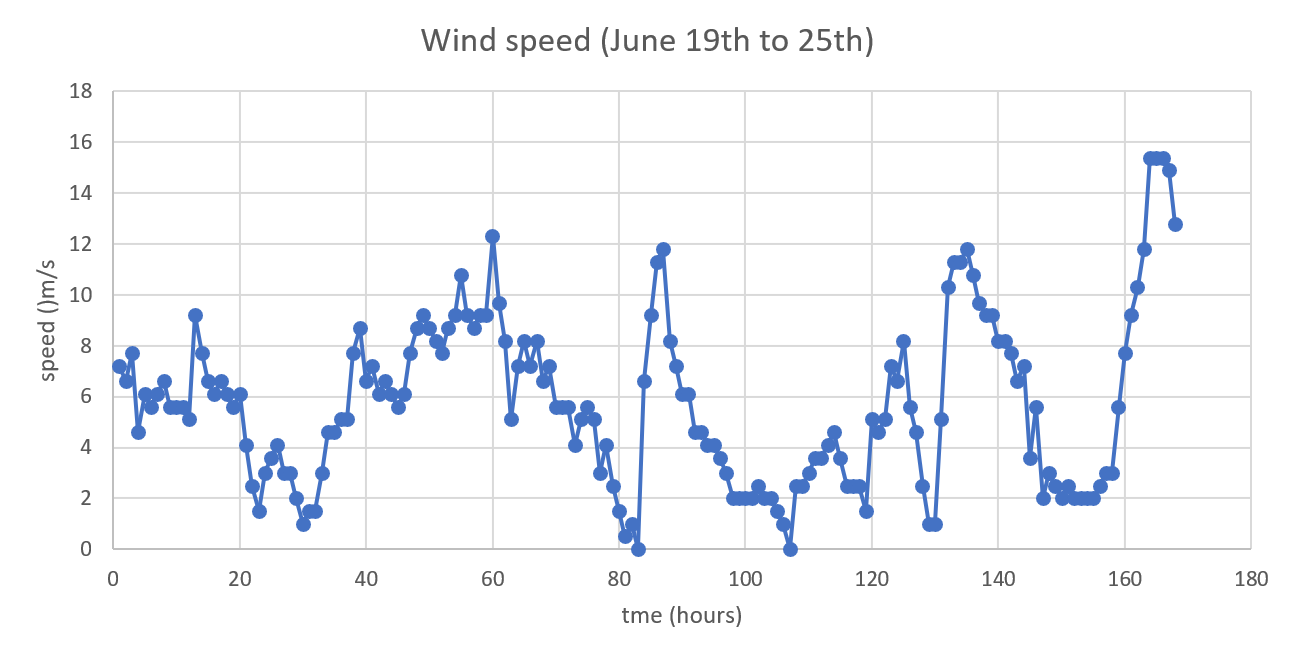
\includegraphics[width=0.5\textwidth]{fig/windspeed.png}
        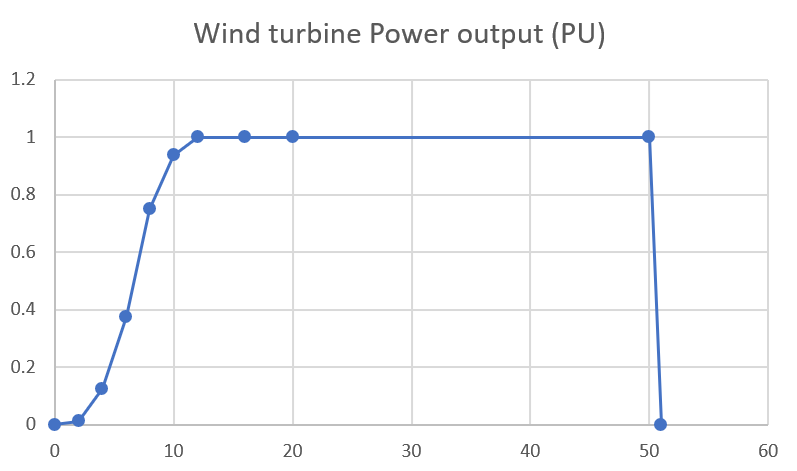
\includegraphics[width=0.5\textwidth]{fig/turbineresp.png}
        \label{ap:wind}

        \newpage
        \section{Nano Sizing Tables}
        \begin{table}[h!]
                \begin{tabular}{|l|l|l|l|l|l|l|l|l|}
                \hline
                \rowcolor[HTML]{C0C0C0} 
                \multicolumn{9}{|c|}{\cellcolor[HTML]{C0C0C0}\textit{\textbf{Initial   Solar}}}                                                                                                                                          \\ \hline
                \textbf{House} & \textbf{daily usage (kWh)} & \textbf{Peak Hrs} & \textbf{PV (kW)} & \textbf{PV cost (\$)}   & \textbf{storage (Ahr)} & \textbf{storage cost (\$)} & \textbf{Total cost (\$)} & \textbf{unserviced (\%)} \\ \hline
                \rowcolor[HTML]{9AFF99} 
                2              & 17.88                      & 2.148857143       & 8.320702034      & \$            21,633.83 & 74.5                   & \$             834.40      & \$    22,468.23          & 12.68                    \\ \hline
                \rowcolor[HTML]{FFFFC7} 
                3              & 19.78                      & 2.148857143       & 9.204892966      & \$            23,932.72 & 82.41666667            & \$             923.07      & \$    24,855.79          & 15.73                    \\ \hline
                \rowcolor[HTML]{FFCCC9} 
                4              & 16                         & 2.148857143       & 7.445818375      & \$            19,359.13 & 66.66666667            & \$             746.67      & \$    20,105.79          & 15.84                    \\ \hline
                \rowcolor[HTML]{CBCEFB} 
                5              & 39.59                      & 2.148857143       & 18.42374684      & \$            47,901.74 & 164.9583333            & \$          1,847.53       & \$    49,749.28          & 6.01                     \\ \hline
                \end{tabular}
        \end{table}
                
        \begin{table}[h!]
                        \begin{tabular}{|l|l|l|l|l|l|l|l|l|}
                        \hline
                        \rowcolor[HTML]{C0C0C0} 
                        \multicolumn{9}{|c|}{\cellcolor[HTML]{C0C0C0}\textit{\textbf{Initial   Wind}}}                                                                                                                                                   \\ \hline
                        \textbf{House} & \textbf{daily usage (kWh)} & \textbf{Peak Hrs} & \textbf{Turbine (kW)} & \textbf{turbine cost (\$)} & \textbf{storage (Ahr)} & \textbf{storage cost (\$)} & \textbf{Total cost (\$)} & \textbf{unserviced (\%)} \\ \hline
                        \rowcolor[HTML]{9AFF99} 
                        2              & 17.88                      & 9.4383            & 1.894408951           & \$            12,578.88    & 74.5                   & \$             834.40      & \$    13,413.28          & 4.672                    \\ \hline
                        \rowcolor[HTML]{FFFFC7} 
                        3              & 19.78                      & 9.4383            & 2.09571639            & \$            13,915.56    & 82.41666667            & \$             923.07      & \$    14,838.62          & 6.8                      \\ \hline
                        \rowcolor[HTML]{FFCCC9} 
                        4              & 16                         & 9.4383            & 1.695220538           & \$            11,256.26    & 66.66666667            & \$             746.67      & \$    12,002.93          & 7.906                    \\ \hline
                        \rowcolor[HTML]{CBCEFB} 
                        5              & 39.59                      & 9.4383            & 4.194611318           & \$            27,852.22    & 164.9583333            & \$          1,847.53       & \$    29,699.75          & 2.596                    \\ \hline
                        \end{tabular}
        \end{table}
        
        \begin{table}[h!]
                                \begin{tabular}{|l|l|l|l|l|l|l|l|l|}
                                \hline
                                \rowcolor[HTML]{C0C0C0} 
                                \multicolumn{9}{|c|}{\cellcolor[HTML]{C0C0C0}\textit{\textbf{Sized   Solar}}}                                                                                                                                            \\ \hline
                                \textbf{House} & \textbf{daily usage (kWh)} & \textbf{Peak Hrs} & \textbf{PV (kW)} & \textbf{PV cost (\$)}   & \textbf{storage (Ahr)} & \textbf{storage cost (\$)} & \textbf{Total cost (\$)} & \textbf{unserviced (\%)} \\ \hline
                                \rowcolor[HTML]{9AFF99} 
                                2              & 17.88                      & 2.148857143       & 10               & \$            26,000.00 & 95                     & \$          1,064.00       & \$    27,064.00          & 3.6                      \\ \hline
                                \rowcolor[HTML]{FFFFC7} 
                                3              & 19.78                      & 2.148857143       & 12               & \$            31,200.00 & 100                    & \$          1,120.00       & \$    32,320.00          & 2.6                      \\ \hline
                                \rowcolor[HTML]{FFCCC9} 
                                4              & 16                         & 2.148857143       & 10               & \$            26,000.00 & 85                     & \$             952.00      & \$    26,952.00          & 3.64                     \\ \hline
                                \rowcolor[HTML]{CBCEFB} 
                                5              & 39.59                      & 2.148857143       & 20               & \$            52,000.00 & 180                    & \$          2,016.00       & \$    54,016.00          & 1.9                      \\ \hline
                                \end{tabular}
        \end{table} 
        
        \begin{table}[h!]
        \begin{tabular}{|l|l|l|l|l|l|l|l|l|}
        \hline
        \rowcolor[HTML]{C0C0C0} 
        \multicolumn{9}{|c|}{\cellcolor[HTML]{C0C0C0}\textit{\textbf{Sized   Wind}}}                                                                                                                                                     \\ \hline
        \textbf{House} & \textbf{daily usage (kWh)} & \textbf{Peak Hrs} & \textbf{Turbine (kW)} & \textbf{turbine cost (\$)} & \textbf{storage (Ahr)} & \textbf{storage cost (\$)} & \textbf{Total cost (\$)} & \textbf{unserviced (\%)} \\ \hline
        \rowcolor[HTML]{9AFF99} 
        2              & 17.88                      & 9.4383            & 2                     & \$            13,280.00    & 80                     & \$             896.00      & \$    14,176.00          & 2.68                     \\ \hline
        \rowcolor[HTML]{FFFFC7} 
        3              & 19.78                      & 9.4383            & 2.6                   & \$            17,264.00    & 95                     & \$          1,064.00       & \$    18,328.00          & 3.2                      \\ \hline
        \rowcolor[HTML]{FFCCC9} 
        4              & 16                         & 9.4383            & 1.8                   & \$            11,952.00    & 85                     & \$             952.00      & \$    12,904.00          & 4.031                    \\ \hline
        \rowcolor[HTML]{CBCEFB} 
        5              & 39.59                      & 9.4383            & 4.5                   & \$            29,880.00    & 165                    & \$          1,848.00       & \$    31,728.00          & 1.79                     \\ \hline
        \end{tabular}
        \end{table}
        \label{ap:nanosize}
        
        \section{Mini Sizing Tables}
        \begin{table}[h!]
                \begin{tabular}{|l|l|l|l|l|l|l|l|l|}
                \hline
                \rowcolor[HTML]{C0C0C0} 
                \multicolumn{9}{|c|}{\cellcolor[HTML]{C0C0C0}\textit{\textbf{Sized   Wind}}}                                                                                                                                                     \\ \hline
                \textbf{House} & \textbf{daily usage (kWh)} & \textbf{Peak Hrs} & \textbf{Turbine (kW)} & \textbf{turbine cost (\$)} & \textbf{storage (Ahr)} & \textbf{storage cost (\$)} & \textbf{Total cost (\$)} & \textbf{unserviced (\%)} \\ \hline
                \rowcolor[HTML]{9AFF99} 
                2              & 17.88                      & 9.4383            & 2                     & \$            13,280.00    & 80                     & \$             896.00      & \$    14,176.00          & 2.68                     \\ \hline
                \rowcolor[HTML]{FFFFC7} 
                3              & 19.78                      & 9.4383            & 2.6                   & \$            17,264.00    & 95                     & \$          1,064.00       & \$    18,328.00          & 3.2                      \\ \hline
                \rowcolor[HTML]{FFCCC9} 
                4              & 16                         & 9.4383            & 1.8                   & \$            11,952.00    & 85                     & \$             952.00      & \$    12,904.00          & 4.031                    \\ \hline
                \rowcolor[HTML]{CBCEFB} 
                5              & 39.59                      & 9.4383            & 4.5                   & \$            29,880.00    & 165                    & \$          1,848.00       & \$    31,728.00          & 1.79                     \\ \hline
                \end{tabular}
        \end{table}

        

\newpage
\nocite{*}
\bibliography{ref}
\bibliographystyle{IEEEtran}
\end{document}
